\begin{figure}
    % \captionsetup[subfigure]{labelformat=empty, size=\large, labelfont={black, bf}}
    \captionsetup[subfigure]{labelformat=empty, font={large, color=black}}
    \begin{subfigure}{0.23\textwidth}
        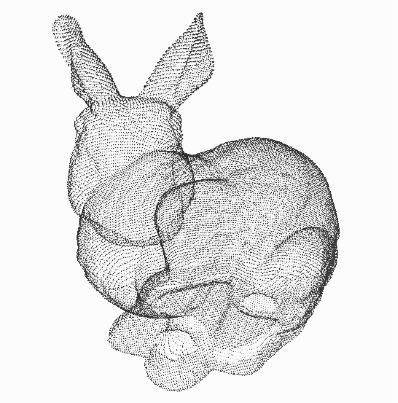
\includegraphics[height=0.35\textheight]{p04_12}
        \caption{Point Cloud}
    \end{subfigure}
    \begin{subfigure}{0.23\textwidth}
        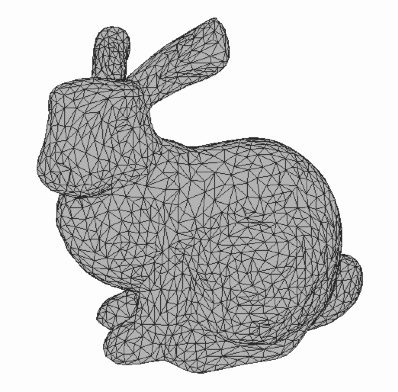
\includegraphics[height=0.35\textheight]{p04_13}
        \caption{Mesh}
    \end{subfigure}
    \begin{subfigure}{0.23\textwidth}
        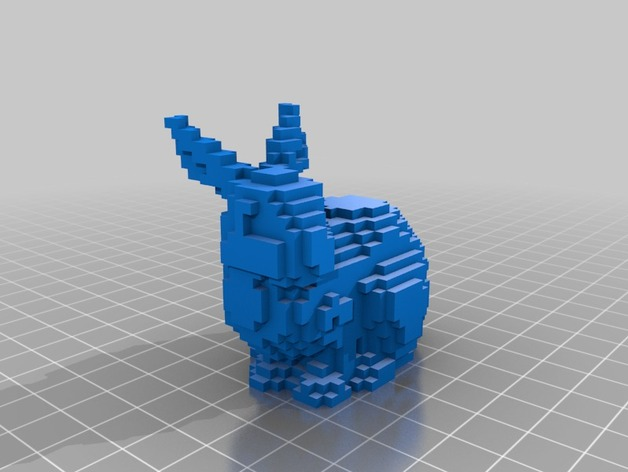
\includegraphics[height=0.35\textheight]{p04_14}
        \caption{Volumetric}
    \end{subfigure}
    \hspace{1mm}
    \begin{subfigure}{0.23\textwidth}
        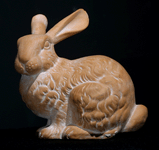
\includegraphics[height=0.35\textheight]{p04_15}
        \caption{View Rendering}
    \end{subfigure}
    \blfootnote{Figures and captions (partially) from CVPR presentation to \cite{qi2017pointnet}.}
\end{figure}
